This section provides a brief introduction to Ethereum v1.0, a
decentralized, open-source blockchain platform that has revolutionized
the field of distributed computing. While Bitcoin introduced the world
to the concept of a peer-to-peer electronic cash system, Ethereum
expanded on this vision by creating a general-purpose blockchain that
enables developers to build and deploy a wide range of decentralized
applications (DAPPs) and smart contracts.

We will begin by exploring the historical context and motivation behind
the creation of Ethereum, including the limitations of Bitcoin's
scripting language that inspired Vitalik Buterin and Gavin Wood to propose a more
flexible and expressive platform. We will then delve into the core
concepts that define the Ethereum ecosystem, such as the Ethereum
Virtual Machine (EVM), the account-based model, and the concept of gas,
which is used to meter the computational resources of the network.

A significant portion of this section will be dedicated to understanding
the technical underpinnings of Ethereum, including the structure of
transactions and blocks, and the use of Merkle-Patricia trees to
efficiently store and verify the global state of the network. By the end
of this section, you will have a solid understanding of the fundamental
principles of Ethereum and the key technological innovations that have
made it the leading platform for smart contracts and decentralized
applications.

\subsection{Learning Objectives}\label{learning-objectives}

\begin{itemize}
	\tightlist
	\item
	Understand the concept of smart contracts and their potential
	applications.
	\item
	Learn about the history and motivation behind the creation of
	Ethereum.
	\item
	Grasp the key features of the Ethereum platform, including its
	Turing-complete scripting language and the Ethereum Virtual Machine
	(EVM).
	\item
	Understand the Ethereum account model and how it differs from
	Bitcoin's UTXO model.
	\item
	Learn about the concept of gas and its role in preventing abuse of the
	network.
	\item
	Gain insight into the structure of Ethereum transactions and blocks.
	\item
	Understand the purpose and function of the Merkle-Patricia Tree in
	managing Ethereum's global state.
\end{itemize}

\begin{center}\rule{0.5\linewidth}{0.5pt}\end{center}

\subsection{The Motivation for Smart
	Contracts}\label{section-1-the-motivation-for-smart-contracts}

\subsubsection{From Legal Contracts to Smart
	Contracts}\label{from-legal-contracts-to-smart-contracts}

Traditional legal contracts, while a cornerstone of modern commerce, are
often fraught with inefficiencies. They can be slow to draft, expensive
to enforce, and subject to the ambiguities of human language. In 1994,
long before the advent of blockchain technology, computer scientist and
cryptographer Nick Szabo envisioned a more efficient and secure
alternative: the \textbf{smart contract}.

Szabo defined a smart contract as a computerized transaction protocol
that executes the terms of a contract. The primary objectives of this
concept were to:

\begin{itemize}
	\tightlist
	\item
	\textbf{Automate Contractual Obligations}: To automatically enforce
	the terms of an agreement, such as payment terms, without the need for
	manual intervention.
	\item
	\textbf{Minimize Exceptions}: To reduce the risk of both malicious and
	accidental exceptions by encoding the terms of the contract in a
	deterministic and unambiguous programming language.
	\item
	\textbf{Reduce Reliance on Trusted Intermediaries}: To minimize the
	need for trusted third parties, such as lawyers and escrow agents,
	thereby reducing transaction costs and increasing efficiency.
\end{itemize}

%A classic example illustrating the need for such automation is an
%\textbf{escrow} service. When buying a house, a significant problem is
%determining the order of operations: should the buyer pay first, or
%should the seller transfer the property title first? An escrow service,
%a trusted third party, solves this by holding the buyer's funds until
%the title transfer is complete. Smart contracts aim to replace such
%intermediaries with automated, trustless code.

\subsubsection{The Limitations of Bitcoin
	Script}\label{the-limitations-of-bitcoin-script}

The Bitcoin protocol, with its simple, stack-based scripting language,
provided the first glimpse of the potential of smart contracts. Bitcoin
Script allows for the creation of basic spending conditions, such as
multi-signature transactions and time-locked payments. However, the
language is intentionally limited in its functionality -- it is not
Turing-complete -- to prioritize security and prevent complex,
potentially malicious scripts from being executed on the network. However, a simple stack-based automaton is insufficient
for Turing-completeness; a more powerful mechanism is required.

This limitation, while a sensible design choice for a digital currency,
made it difficult to build more complex and sophisticated applications
on top of the Bitcoin blockchain. The need for a more general-purpose
blockchain platform with a Turing-complete scripting language was the
primary motivation for the creation of Ethereum.

\begin{center}\rule{0.5\linewidth}{0.5pt}\end{center}

\subsection{An Introduction to
	Ethereum}\label{section-2-an-introduction-to-ethereum}

\subsubsection{The Vision of a World
	Computer}\label{the-vision-of-a-world-computer}

Launched in 2015, Ethereum was conceived with the ambitious vision of
creating a ``world computer'' -- a single, decentralized platform capable
of running any application. This vision was a direct response to the
limitations of Bitcoin, which, while revolutionary, was primarily
designed as a peer-to-peer electronic cash system. Ethereum, in
contrast, was designed to be a general-purpose blockchain, providing
developers with the tools and flexibility to build and deploy their own
smart contracts and decentralized applications (DAPPs).
The key features that enable this vision include:

\begin{itemize}
	\tightlist
	\item
	\textbf{Quasi-Turing-complete Smart Contracts}: Ethereum's primary
	programming language, Solidity, is often described as Turing-complete,
	meaning it can compute anything that is computable. However, this is
	practically limited by the concept of ``gas'' to prevent infinite
	loops. This allows for the creation of sophisticated DAPPs that can
	automate a wide range of processes and interactions.
	\item
	\textbf{The Ethereum Virtual Machine (EVM)}: The EVM is the runtime
	environment for smart contracts on the Ethereum network. It is a
	sandboxed virtual machine that is completely isolated from the host
	node's network, filesystem, or processes, ensuring that smart
	contracts are executed in a secure and deterministic manner.
	\item
	\textbf{Decentralized Finance (DeFi)}: Ethereum's flexible and
	expressive smart contract capabilities have made it the leading
	platform for the burgeoning field of Decentralized Finance (DeFi).
	DeFi applications aim to recreate traditional financial services, such
	as lending, borrowing, and trading, in a decentralized and
	permissionless manner.
\end{itemize}

\subsubsection{The Ethereum Account
	Model}\label{the-ethereum-account-model}

A key architectural difference between Bitcoin and Ethereum is their
respective account models. While Bitcoin uses the \textbf{Unspent
	Transaction Output (UTXO)} model, Ethereum employs an
\textbf{account-balance-based model}, which is more analogous to a traditional
bank account. There are two types of accounts in Ethereum:

\begin{itemize}
	\tightlist
	\item
	\textbf{Externally Owned Accounts (EOAs)}: These accounts are
	controlled by users via their private keys. EOAs can send transactions
	to other accounts and can trigger the execution of smart contracts.
	\item
	\textbf{Contract Accounts}: These accounts are controlled by the code
	of a smart contract. A contract account is created when a smart
	contract is deployed to the blockchain, and it can only execute code
	in response to a transaction or a message call from another account.
\end{itemize}

Each Ethereum account is associated with a unique 20B-long address and maintains
a state that includes its balance of Ether (ETH), the native
cryptocurrency of the Ethereum network, as well as a \textbf{nonce} (a
transaction counter to prevent replay attacks), a \textbf{storage root},
and a \textbf{code hash}.
Nonce field has context-based interpretation and based on the account type.
In the case of EOA account, the value of nonce represents the number of transactions sent from this account while in the case of smart contract account, the nonce value represents the number of smart contract creations made by tbe smart contract account.
Note that the code hash stands for the cryptographically hashed EVM bytecode of the smart contract account, while the code fragments are stored in a dedicated state database, under their hashes -- this is to efficiently optimize the storage for the same codes. The code hash field is immutable (unlike other fields).

\subsubsection{The concept of Gas}\label{gas-and-the-ethereum-virtual-machine-evm}

To prevent the network from being bogged down by infinite loops or other
forms of computational abuse, Ethereum incorporates a mechanism known as
\textbf{gas}. Gas is a unit of measurement for the computational effort
required to execute operations on the EVM. Every operation, from a
simple addition to a complex storage write, has a specific gas cost.

When a user sends a transaction, they must specify a \textbf{gas limit},
which is the maximum amount of gas they are willing to pay for the
transaction. They must also specify a \textbf{gas price}, which is the
amount of Ether they are willing to pay per unit of gas. The total cost
of the transaction is the product of the gas used and the gas price.
This system ensures that the network's computational resources are
allocated efficiently and provides a mechanism for compensating miners
for their work. If a transaction runs out of gas, its operations are
reverted, but the fee is still paid to the miner.

The EVM itself is a stack-based virtual machine with a 256-bit word
size. It provides a secure and deterministic environment for executing
smart contracts, ensuring that all nodes in the network will arrive at
the same result when executing the same code.

\paragraph{\textbf{Gas Price.}}
Every instruction of the EVM has a different gas price, mostly depending on whether it modifies storage or works only with memory. 
In general, the operations with volatile memory are cheap while permanent modification to storage are expensive.
See the example of gas prices of various instructions in \autoref{fig:eth-gas-price}, as introduced by the original version of the Ethereum Yellow paper~\cite{wood2014ethereum}. Note that the transfer transactions costs 21k of gas, which is often used as a baseline for comparison with other smart contract calls.


\begin{figure}[t]
	%	\vspace{-0.3cm}
	\begin{center}
		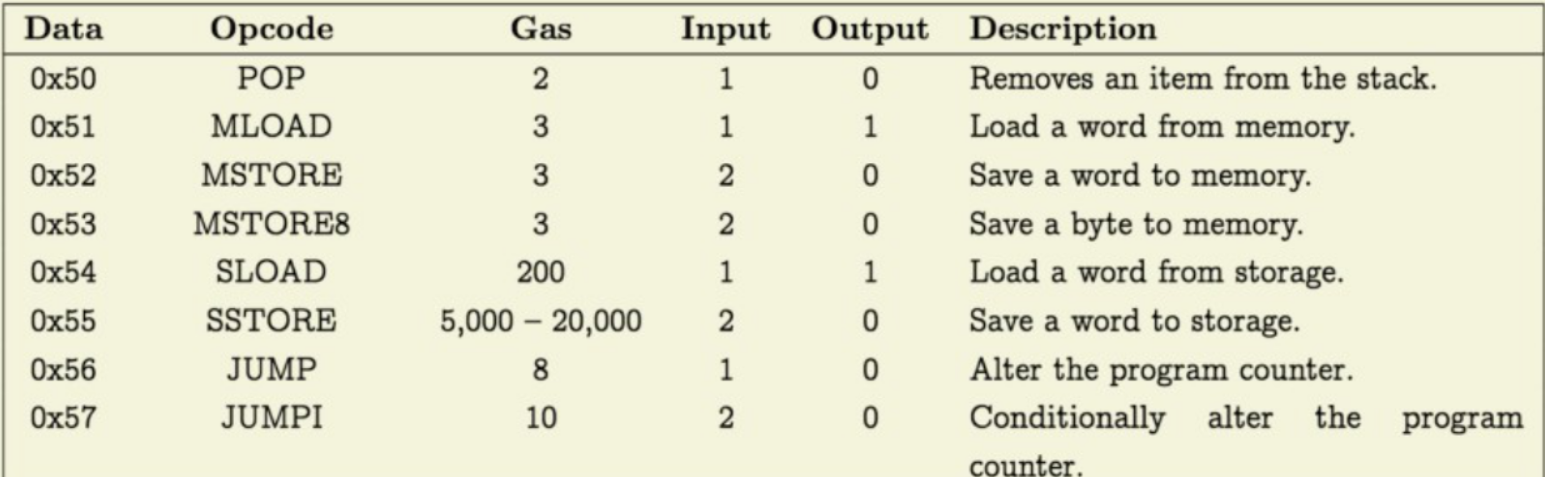
\includegraphics[width=0.9\textwidth]{./figs/gas-price.png}
		\caption{Gas prices of some EVM instructions.}		
		\label{fig:eth-gas-price}
	\end{center}	
\end{figure}

\paragraph{\textbf{Execution of Transaction Calling Smart Contract.}}
The simple pseudocode of deducting gas while doing transaction execution in EVM is described in the following listing:
\begin{enumerate}
	\tightlist
	\item Specify startGas and gasPrice
	\item  Assert(startGas*gasPrice $\leq$ balanceOfCaller)
	\item  balanceOfCaller -= startGas*gasPrice
	\item tmpGas = startGas ; gasRefund = 0
	\item Execute code, deducting from tmpGas
	\begin{itemize}
		\item deducted = ExecutionCost(tx)
		\item \textbf{If} deducted $<$ 0 \textbf{then} \\
		\hspace{0.5cm} ~~~~gasRefund += $|$deducted$|$ \\
		\textbf{else} \\
		\hspace{0.5cm} ~~~~tmpGas -= deducted \\
		\item Assert(tmpGas$\geq$ 0)
	\end{itemize}
	
	\item Refund gasRefund + tmpGas to balanceOfCaller	
\end{enumerate}



\subsubsection{EIP-1559}\label{gas-and-the-ethereum-virtual-machine-evm}
The EIPT-1559 \ih{ref} was included in London's hardfork that occurred on 5th of August 2021, and its main contribution is to optimize the fee market system.
In particular, this EIP introduces 3 elements of gas:
\begin{itemize}
	\item \textbf{Base fee} -- the minimum amount of gas for a transaction, which is burnt. It is set by the network. Blocks can be extended to 200\% of the base fee.
	
	\item \textbf{Tip} -- is set by the user, and it represents a premium to miners that should prioritize the faster inclusion of their transaction.
	
	\item \textbf{Fee cap} -- represents the the maximum amount of gas a user is willing to pay. Therefore, the refund is computed as  fee cap – (base fee + tip).	
\end{itemize}
This EIP improves economics of Ethereum since base we must always be ``payed'' in ETH, while before it could be paid in any currency or token of a the exchange with the full node that handled the fee internally.

\begin{center}\rule{0.5\linewidth}{0.5pt}\end{center}

\subsection{Ethereum Transactions and
	Blocks}\label{section-3-ethereum-transactions-and-blocks}

\subsubsection{Transactions}\label{transactions}

An Ethereum transaction is a cryptographically signed message that is
broadcast to the network and recorded on the blockchain. There are two
fundamental types of transactions in Ethereum:

\begin{enumerate}
	\tightlist
	\item
	\textbf{Contract Creation Transactions}: These transactions are used
	to deploy new smart contracts to the Ethereum blockchain. The
	transaction's data field contains the compiled bytecode of the smart
	contract, which is then executed by the EVM to create the new contract
	account.
	\item
	\textbf{Message Calls}: These transactions are used to interact with
	existing accounts. This can involve transferring Ether from one
	account to another, or it can involve calling a function on a smart
	contract.
\end{enumerate}

Every Ethereum transaction contains several important fields:

\begin{itemize}
	\tightlist
	\item
	\textbf{Nonce}: A sequence number that is used to prevent replay
	attacks.
	\item
	\textbf{Gas Price}: The price per unit of gas that the sender is
	willing to pay.
	\item
	\textbf{Gas Limit}: The maximum amount of gas that the sender is
	willing to use for the transaction.
	\item
	\textbf{To}: The address of the recipient account.
	\item
	\textbf{Value}: The amount of Ether to be transferred.
	\item
	\textbf{Data}: The input data for a message call, or the compiled
	bytecode for a contract creation transaction.
	\item
	\textbf{Signature}: A digital signature that authenticates the sender.
\end{itemize}

\subsubsection{Blocks}\label{blocks}

An Ethereum block is a collection of transactions that are bundled
together and added to the blockchain. Each block consists of a header
and a body. The body contains a list of all the transactions included in
the block, as well as a list of ``\textbf{ommers},'' which are the
headers of stale blocks that were not included in the main chain but are
still rewarded to incentivize miners and improve security.
The block header (of legacy Ethereum v1.0) contains several crucial pieces of information (see also \autoref{fig:eth-eth-header}):

\begin{figure}[t]
	%	\vspace{-0.3cm}
	\begin{center}
		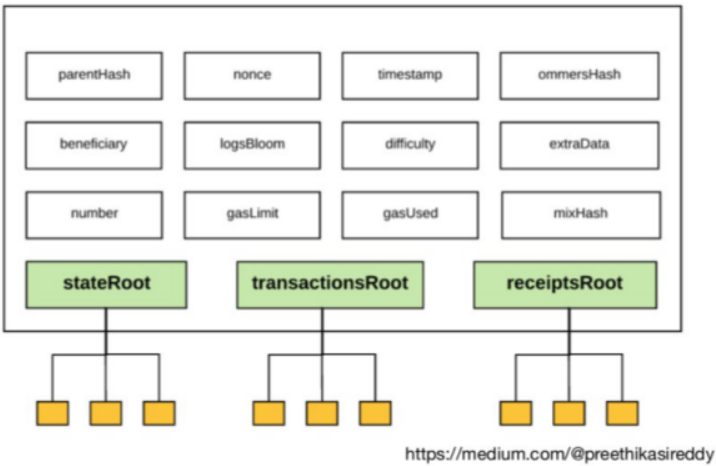
\includegraphics[width=0.7\textwidth]{./figs/eth-block.png}
		\caption{A structure of the header in Ethereum v1.0.}		
		\label{fig:eth-eth-header}
	\end{center}	
\end{figure}


\begin{itemize}
	\tightlist
	\item
	\textbf{Parent Hash}: The hash of the previous block's header, which
	links the blocks together in a chain.
	\item
	\textbf{Block Number}: The sequence number of the block in the chain.
	\item \textbf{Nonce}: replay protection counter.
	\item \textbf{Beneficiary}: the miner of the block -- replaces a coinbase transaction known from Bitcoin.
	\item
	\textbf{Timestamp}: The time at which the block was created.
	\item \textbf{ommersHash}: aggregates stale parent block headers whose miners get a certain partial reward.	
	\item
	\textbf{Difficulty}: The difficulty of the Proof-of-Work puzzle for
	the block.
	\item
	\textbf{Gas Limit and Gas Used}: The maximum amount of gas allowed in
	the block and the total amount of gas used by all the transactions in
	the block.
	\item
	\textbf{State Root, Transaction Root, and Receipt Root}: The root
	hashes of three Merkle-Patricia trees that store the global state, the
	transactions, and the transaction receipts, respectively.
	\item \textbf{ExtraData}: arbitrary data of max. 32B. (e.g., name of the mining pool)
	\item
	\textbf{Logs Bloom}: A Bloom filter that provides an efficient way to
	search for event logs generated by smart contracts within the block.
\end{itemize}

\subsubsection{The Global State and Merkle-Patricia
	Trees}\label{the-global-state-and-merkle-patricia-trees}

The \textbf{global state} of Ethereum is a massive data structure that
contains a mapping of all account addresses to their corresponding
account states. This state is not stored in the blockchain itself, but
rather in a separate key-value database that is maintained by all full
nodes.
The example of a transaction that calls smart contract account and thus changes the state is depicted in \autoref{fig:eth-state-change}.


\begin{figure}[t]
	%	\vspace{-0.3cm}
	\begin{center}
		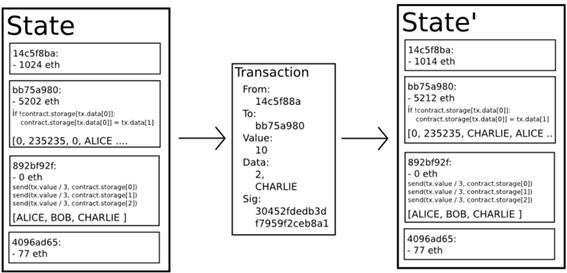
\includegraphics[width=0.7\textwidth]{./figs/eth-state-change.png}
		\caption{A transaction call that changes the state of the smart contract and its value.}		
		\label{fig:eth-state-change}
	\end{center}	
\end{figure}


To efficiently store and verify the global state, Ethereum uses a
sophisticated data structure called a \textbf{Merkle-Patricia Tree
	(MPT)}. The MPT is a hybrid data structure that combines the properties
of a Merkle tree (for integrity) and a Radix/Patricia trie (for
efficient lookups). This allows for efficient verification of the state
and enables light clients to securely query the state of an account
without having to download the entire blockchain. The root of the MPT,
known as the \textbf{state root}, is included in the block header, which
provides a cryptographic commitment to the entire state of the network
at that point in time.
MPT contains 3 types of nodes:
\begin{compactenum}
	\item \textbf{Extension nodes}: aggregate symbols in the key.
	\item \textbf{Branch nodes}: splits the path according to the current symbol in the key.
	\item \textbf{Leaf nodes}: they store data of the account states (or storages).	
\end{compactenum}
The example of ste state trie built using MPT is depicted in \autoref{fig:eth-mpt}, and it contains 4 accounts.

\begin{figure}[t]
	%	\vspace{-0.3cm}
	\begin{center}
		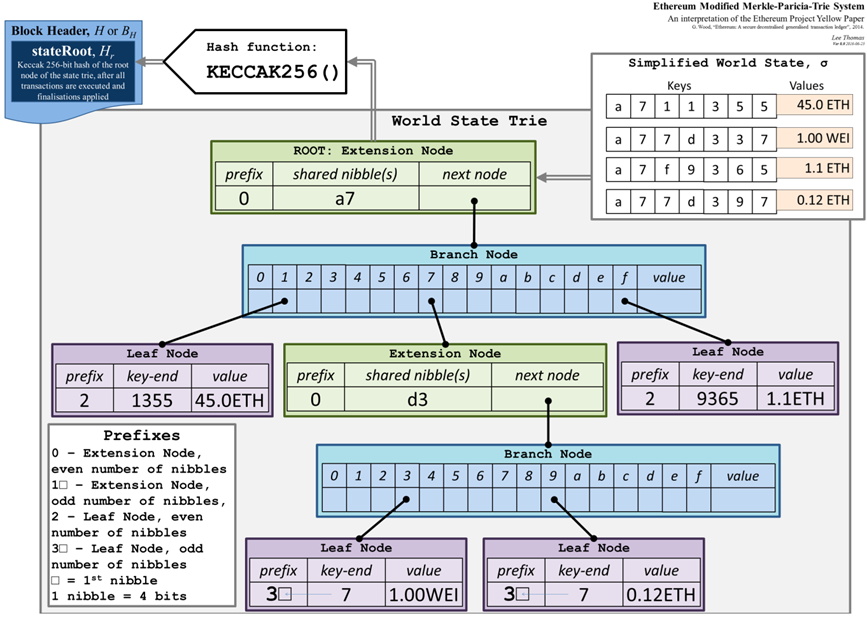
\includegraphics[width=0.95\textwidth]{./figs/eth-mpt.png}
		\caption{A Merkle-Patricia Trie for storing the global state in Ethereum.}		
		\label{fig:eth-mpt}
	\end{center}	
\end{figure}



\subsubsection{Bloom Filters and Transaction
	Receipts}\label{bloom-filters-and-transaction-receipts}

For every transaction, Ethereum generates a \textbf{receipt}, which
contains information about the outcome of the transaction, including the
gas used and, importantly, any \textbf{logs} or events emitted by the
smart contract during its execution.

To allow for efficient searching of these logs without requiring nodes
to scan every transaction in every block, Ethereum uses \textbf{Bloom
	filters}. A Bloom filter is a space-efficient probabilistic data
structure that can quickly test whether an element is a member of a set.
While it can produce false positives, it will never produce a false
negative.

Bloom filter is an $m$ bit array that requires $k$ different (cryptographically insecure) hash functions, where $k << m$. 
Bloom filter supports 2 operations:
\begin{compactenum}
	\item \textbf{Add element} -- we hash new element with k hash functions and set 1 on obtained positions.
	\item \textbf{Query element} -- we hash queried element with k hash functions and if 1 is on all positions, return true. Otherwise, return false (see \autoref{fig:eth-bloom-filter}).
\end{compactenum}
Bloom filter is often use as a pre-filter for expensive storage-lookup queries (see \autoref{fig:bloom-app}).

\begin{figure}[t]
	%	\vspace{-0.3cm}
	\begin{center}
		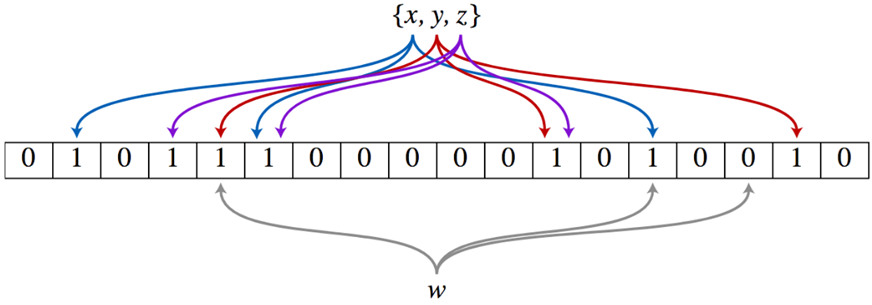
\includegraphics[width=0.9\textwidth]{./figs/bloom.png}
		\caption{An example of the Bloom filter with 3 hashing functions  and 3 elements. Element w in query is not included in the Bloom filter.}		
		\label{fig:eth-bloom-filter}
	\end{center}	
\end{figure}


\begin{figure}[t]
	%	\vspace{-0.3cm}
	\begin{center}
		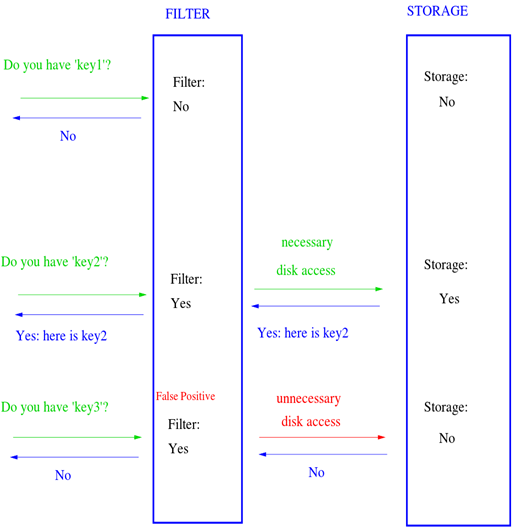
\includegraphics[width=0.7\textwidth]{./figs/bloom-eg.png}
		\caption{Application of Bloom filter for pre-filtering of queries.}		
		\label{fig:bloom-app}
	\end{center}	
\end{figure}



In Ethereum, each transaction receipt contains a Bloom filter of its logs, and the
block header contains a cumulative Bloom filter that aggregates the
filters from all transaction receipts in the block. This allows DAPPs
and light clients to quickly and efficiently find relevant events by
first checking the Bloom filter in the block header.




\begin{center}\rule{0.5\linewidth}{0.5pt}\end{center}

\subsection{Summary / Key Takeaways}\label{summary-key-takeaways}

This section has provided a comprehensive introduction to Ethereum, the
first and currently the most adopted platform for decentralized applications and smart
contracts. We have explored the historical context and motivation behind
its creation, highlighting the limitations of Bitcoin's scripting
language that spurred the development of a more general-purpose
blockchain.

We have delved into the core concepts that define the Ethereum
ecosystem, including:

\begin{itemize}
	\tightlist
	\item
	\textbf{Smart Contracts}: Self-executing contracts with the terms of
	the agreement directly written into code, enabling automation and
	reducing the need for intermediaries.
	\item
	\textbf{The Ethereum Virtual Machine (EVM)}: The sandboxed,
	deterministic runtime environment for smart contracts on the Ethereum
	network.
	\item
	\textbf{The Account-Based Model}: Ethereum's approach to tracking the
	state of the network, which is more intuitive for developers than
	Bitcoin's UTXO model.
	\item
	\textbf{Gas}: The mechanism for metering the computational resources
	of the network, preventing abuse and compensating miners.
	\item
	\textbf{Merkle-Patricia Trees}: The sophisticated data structure used
	to efficiently and securely store the global state of all accounts.
	\item
	\textbf{Bloom Filters}: A probabilistic data structure used to make
	searching for smart contract events highly efficient.
\end{itemize}


\begin{center}\rule{0.5\linewidth}{0.5pt}\end{center}

\subsection{Keywords}\label{keywords}

\begin{itemize}
	\tightlist
	\item
	\textbf{Ethereum}: A decentralized, open-source blockchain platform
	that enables the creation and deployment of smart contracts and
	decentralized applications (DAPPs).
	\item
	\textbf{Smart Contract}: A computer protocol intended to digitally
	facilitate, verify, or enforce the negotiation or performance of a
	contract.
	\item
	\textbf{Ethereum Virtual Machine (EVM)}: The runtime environment for
	smart contracts in Ethereum. It is a quasi-Turing-complete virtual
	machine that executes code as a sandboxed process.
	\item
	\textbf{Gas}: The unit of measurement for the computational effort
	required to execute operations on the Ethereum network.
	\item
	\textbf{Account Model}: An account model used in Ethereum where the
	state of the blockchain is represented as a set of accounts, each with
	its own balance, storage, and code.
	\item
	\textbf{Merkle-Patricia Tree (MPT)}: A hybrid data structure that
	combines a Merkle tree and a Patricia trie to efficiently store and
	verify the global state of the Ethereum network.
	\item
	\textbf{Externally Owned Account (EOA)}: An Ethereum account that is
	controlled by a user's private key.
	\item
	\textbf{Contract Account}: An Ethereum account that is controlled by
	the code of a smart contract.
	\item
	\textbf{Decentralized Finance (DeFi)}: A new financial system built on
	public blockchains that provides an alternative to traditional
	financial services.
	\item
	\textbf{Bloom Filter}: A space-efficient probabilistic data structure
	used in Ethereum to facilitate fast queries for log events.
\end{itemize}

\begin{center}\rule{0.5\linewidth}{0.5pt}\end{center}

\subsection{Further Reading}\label{further-reading}

\begin{itemize}
	\tightlist
	\item
	\textbf{Ethereum White Paper}: \\ 
	\url{https://ethereum.org/en/whitepaper/}
	\item
	\textbf{Ethereum Yellow Paper}: \\
	\url{https://ethereum.github.io/yellowpaper/paper.pdf}
	\item
	\textbf{Mastering Ethereum by Andreas M. Antonopoulos and Gavin Wood}: \\
	\url{https://github.com/ethereumbook/ethereumbook}
\end{itemize}
